% Latex template: mahmoud.s.fahmy@students.kasralainy.edu.eg
% For more details: https://www.sharelatex.com/learn/Beamer

\documentclass{beamer}					% Document class

\setbeamertemplate{footline}[text line]{%
  \parbox{\linewidth}{\vspace*{-8pt}Feature Selection with Mutual Information\hfill\insertshortauthor\hfill\insertpagenumber}}
\setbeamertemplate{navigation symbols}{}

\usepackage[english]{babel}				% Set language
\usepackage[utf8x]{inputenc}			% Set encoding

\mode<presentation>						% Set options
{
  \usetheme{default}					% Set theme
  \usecolortheme{default} 				% Set colors
  \usefonttheme{default}  				% Set font theme
  \setbeamertemplate{caption}[numbered]	% Set caption to be numbered
}

% Uncomment this to have the outline at the beginning of each section highlighted.
%\AtBeginSection[]
%{
%  \begin{frame}{Outline}
%    \tableofcontents[currentsection]
%  \end{frame}
%}

\usepackage{graphicx}					% For including figures
\usepackage{booktabs}					% For table rules
\usepackage{hyperref}					% For cross-referencing
\usepackage{bm}
\usepackage{algorithm,algorithmic}

\title{Feature Selection with Mutual Information}	% Presentation title
\author{Clayton W. Seitz}								% Presentation author
\date{\today}									% Today's date	

\begin{document}

% Title page
% This page includes the informations defined earlier including title, author/s, affiliation/s and the date
\begin{frame}
  \titlepage
\end{frame}

% Outline
% This page includes the outline (Table of content) of the presentation. All sections and subsections will appear in the outline by default.
\begin{frame}{Outline}
  \tableofcontents
\end{frame}

% The following is the most frequently used slide types in beamer
% The slide structure is as follows:
%
%\begin{frame}{<slide-title>}
%	<content>
%\end{frame}

\begin{frame}{Feature Selection}

Why do we perform feature selection? \\
\vspace{0.2in}
\begin{itemize}
\item Quality of the input data is just as important as the algorithm you choose
\item The volume of a feature space grows exponentially in the number of dimensions $V \propto \alpha^{N}$
\item But we often have a small number of samples
\end{itemize}

\end{frame}


\begin{frame}{Using Mutual Information for Feature Selection}

Mutual information comes from information theory and statistics.

\begin{align*}
I(X;Y) &= D_{KL}(P(X,Y)||P(X)P(Y))\\
&= H(X) - H(X|Y)
\end{align*}

where $H$ denotes the entropy\\
\vspace{0.1in}

\begin{itemize}
\item It quantifies the amount of information one variable carries about another
\item Is a ``generalized correlation'' - it is not limited to continuous random variables
\item $X = \{x_{i}\}_{i=1}^{N}$ and $Y$ could be categorical e.g., cellular phenotypes
\end{itemize}

\end{frame}

\begin{frame}{Using Mutual Information for Feature Selection}

For phenotyping, we might want to find the optimal $X$ which is most informative about the cell type $Y$\\
\vspace{0.2in}
This is just an optimization problem on maximizing the joint mutual information

\begin{equation*}
X^{*} = \underset{X}{\mathrm{argmax}}\;\; I(\bm{X};Y)
\end{equation*}

But this is a NP-hard optimization problem, but there are approximate solutions

\end{frame}

\begin{frame}{Results for T1D dataset}

Maximize:
\begin{align*}
I(\bm{X};Y) &\approx \sum_{i} \left(I(X_{i};Y)- \alpha\sum_{j}I(X_{i};X_{j}) \right)
\end{align*}

\begin{center}
\begin{figure}
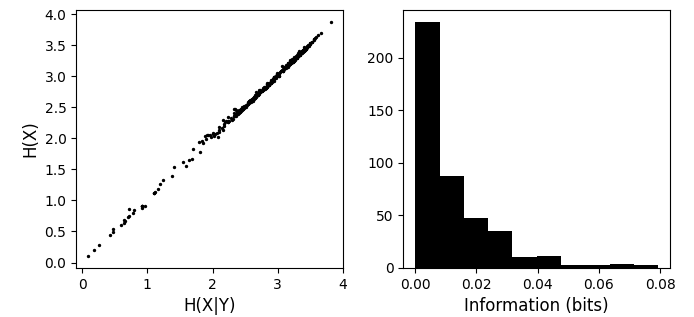
\includegraphics[width=1.0\textwidth]{info.png}
\end{figure}
\end{center}
\end{frame}

\begin{frame}{Algorithm Details}

The chain-rule for mutual information tells us that

\begin{equation}
I(\bm{X};Y) = \sum_{i}I(X_{i};Y|\bm{X}_{\backslash i})
\end{equation} 

To simplify notation let $Z = \bm{X}_{\backslash i}$. The chain rule for info can also be used to show that 

\begin{equation*}
I(X;Y,Z) = I(X;Z) + I(X;Y|Z)
\end{equation*}

Solving for $I(X;Y|Z)$ says we can rewrite (1) as

\begin{align*}
I(\bm{X};Y) &= \sum_{i}I(X_{i};Y|Z)\\
&= \sum_{i}I(X_{i};Y,Z) - I(X_{i};Z)
\end{align*} 

\end{frame}

\begin{frame}{Algorithm Details}

Applying the chain rule one more time gives

\begin{align*}
I(\bm{X};Y) &= \sum_{i}I(X_{i};Y,Z) - I(X_{i};Z)\\
&= \sum_{i}I(X_{i};Y)- I(X_{i};Z) + I(X_{i};Z|Y)
\end{align*} 


We maximize the sum by maximizing the each term $s_{i}$

\begin{align*}
s_{i} &= I(X_{i};Y)- I(X_{i};Z) + I(X_{i};Z|Y)\\
&\approx I(X_{i};Y)- \alpha\sum_{j}I(X_{i};X_{j}) + \beta\sum_{k}I(X_{i};X_{k}|Y)
\end{align*}

Setting $\beta=0$ gives the so-called maximum relevancy minimum redundancy (MRMR) features

\end{frame}

\begin{frame}{Algorithm Details}

\begin{align*}
s_{i} &\approx I(X_{i};Y)- \alpha\sum_{j}I(X_{i};X_{j}) 
\end{align*}

\begin{algorithm}[H]
\begin{algorithmic}[1]
\STATE $features = \{\}$
\FOR{$i=1$ to $N$}
  \IF{$i=1$}
    \STATE add $x_{i}$ to features
  \ELSE
  \IF{$s_{i}>s_{i-1}$}
    \STATE add $x_{i}$ to features
  \ENDIF
  \ENDIF
\ENDFOR
\end{algorithmic}
\caption{Pseudocode for Greedy MRMR}
\label{alg:seq}
\end{algorithm}

\end{frame}



\section{References}

% Adding the option 'allowframebreaks' allows the contents of the slide to be expanded in more than one slide.
\begin{frame}[allowframebreaks]{References}
	\tiny\bibliography{references}
	\bibliographystyle{apalike}
\end{frame}

\end{document}